\subsection{NMF Synchronizations}
\label{sec:NMF}

\emph{NMF Synchronizations}~\cite{SoSyM2017-Hinkel} is a bx language realized as an internal domain-specific language with C\# as a host language.
To program a bx with NMF Synchronizations, a transformation developer specifies a set of consistency relations between the elements of the source and target models.
Starting with a top-most relation, representing the consistency of the entire models, each relation can ``invoke'' other relations, which must hold for this relation to be satisfied.
Leaf relations can be, for example, identity of primitive types such as strings.

This coupling of relations is specified with so called \emph{synchronization blocks},  one of which is depicted schematically in figure~\ref{fig:SynchronizationBlock}.
The relations are represented by horizontal arrows: $\varPhi_{A-C}$ between source elements of type $A$ and target elements of type $C$, and $\varPhi_{B-D}$ between source elements of type $B$ and target elements of type $D$.
The \emph{base relation}  $\varPhi_{A-C}$ holds only if the \emph{target relation} $\varPhi_{B-D}$ holds for certain pairs of $(B,D)$ elements, determined by the \emph{intra-model lenses} $f$ and $g$ (depicted as vertical arrows in figure~\ref{fig:SynchronizationBlock}).

A target relation may occur as base relation in another synchronization block, resulting in nested synchronization blocks.
Furthermore, a relation may play the role of a base relation in multiple synchronization blocks, meaning that multiple consistency relations are required for making a pair of elements in the base relation consistent.

\begin{figure}[b!]
	\centering
	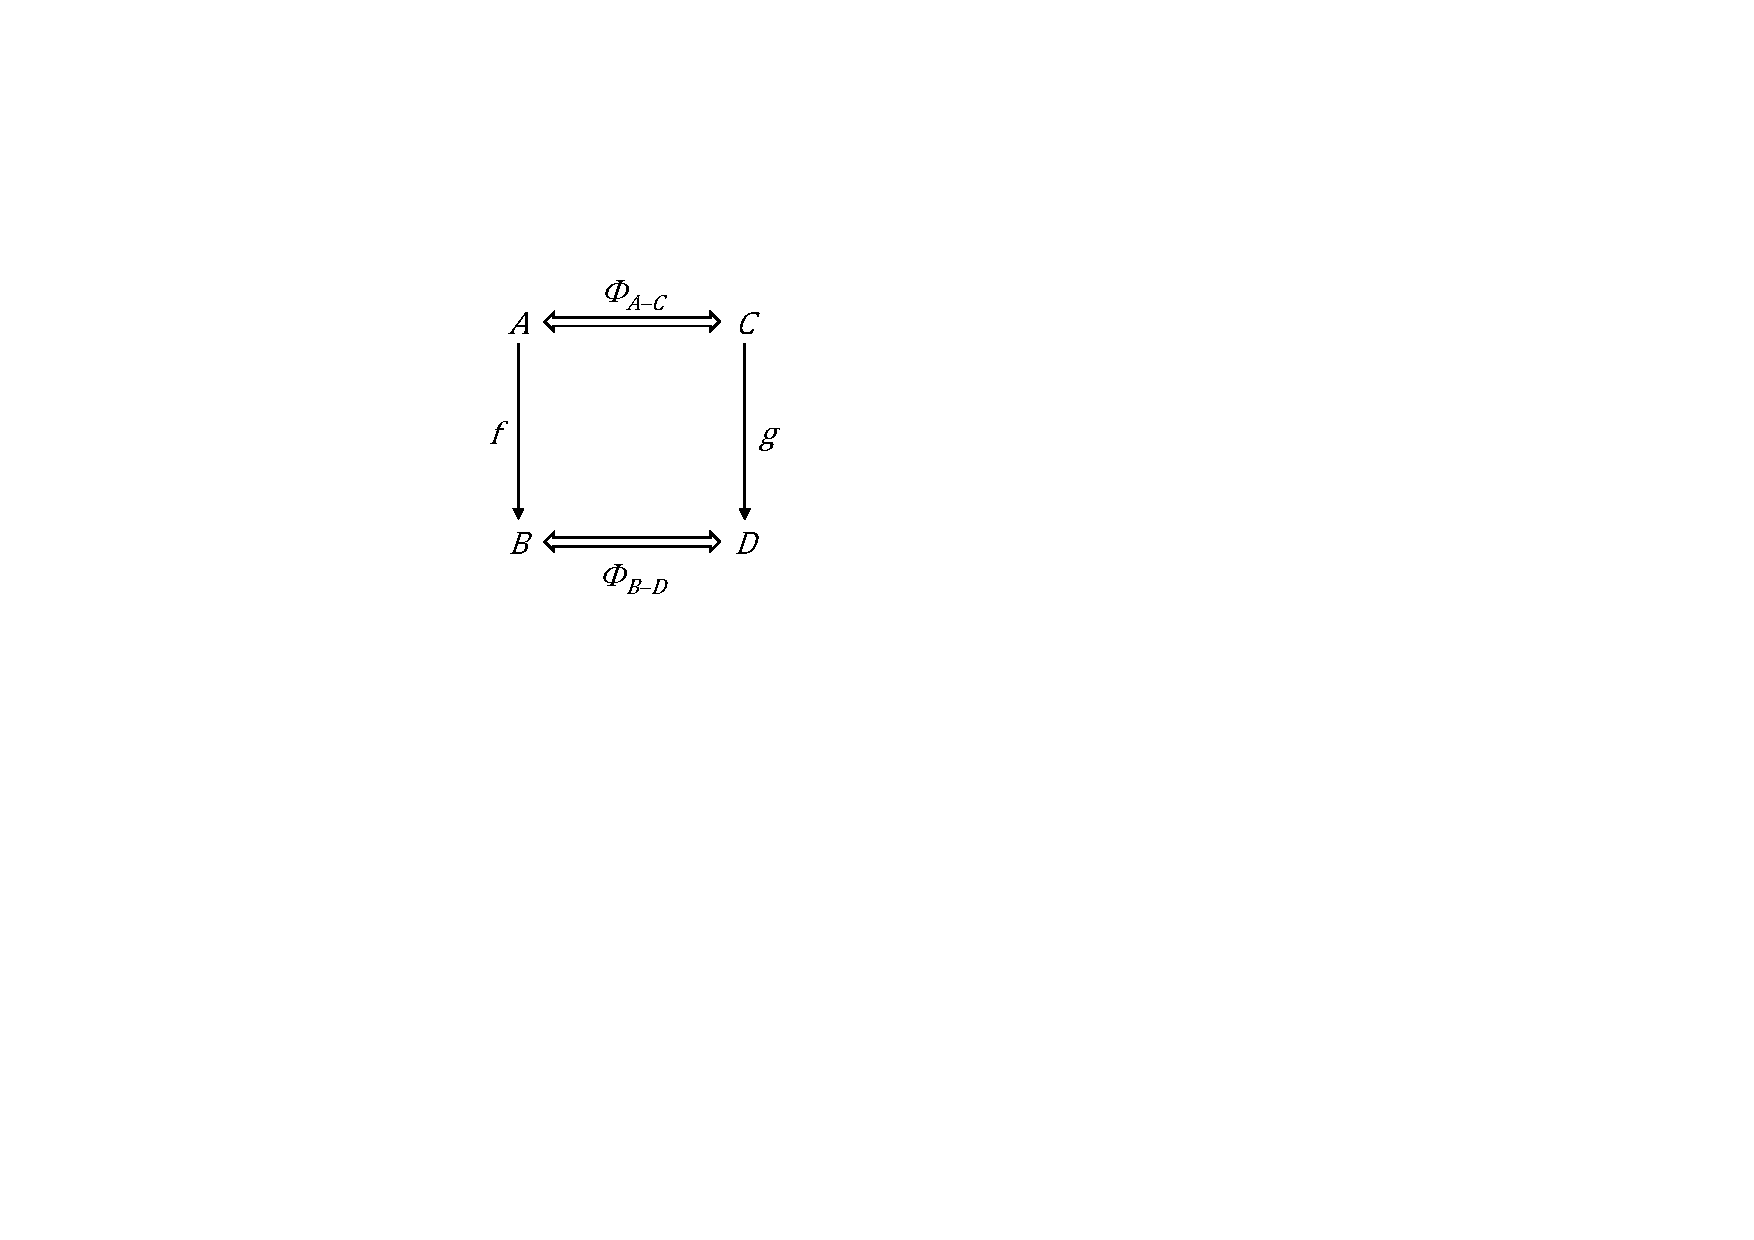
\includegraphics[width=0.35\columnwidth]{diagrams/solutions/NMFSynchronizationBlock}
	\caption{Schematic view of a synchronization block}
	\label{fig:SynchronizationBlock}
\end{figure}

The intra-model lenses $f$ and $g$ are each composed of a \emph{get} and a \emph{put} function:  $f.get: A \rightarrow B, g.get: C \rightarrow D$, and $f.put: A \times B \rightarrow A, g.put:  C \times D \rightarrow D$.

As described above, the \emph{get} function is a simple model query indicating how the base and target relations are coupled, i.e., for which elements the target relation must hold with respect to a given pair of elements in the base relation.
In the simplest cases, this can be a getter navigating to the properties or contained children of an object.

The \emph{put} functions implement updates, i.e., a way of propagating changes of elements in the target relation back to elements in the base relation.
As synchronization blocks pair such updates, they can be viewed as an implementation of update propagation (\emph{fUP} and \emph{bUP}).

\subsubsection{Classification}
\label{sec:ClassificationNMF}

As synchronization blocks can be viewed as pairs of updates (and queries), the style of specification is probably closest to \emph{propagataion-based}.
%
The addressed application scenario is \emph{o-delta-corr-based}: the NMF solution accepts o-deltas and a corr as vertical and horizontal input, respectively.
%
Hinkel et al.~\cite{SoSyM2017-Hinkel} provide a proof for \emph{correctness} and \emph{hippocraticness} under the assumption that the transformation developer ensures that \emph{get-put} and \emph{put-get} laws are actually satisfied for all intra-model lenses.
%
The consistency relation between two models is specified \emph{explicitly} by a set of coupled synchronization blocks, using only the \emph{get} operations.
This combination of relations coupled by queries is similar to a JTL program and can be best viewed as a \emph{constraint-based} specification of consistency. 

Consistency restoration is implemented by providing corresponding \emph{put} operations for each synchronization block.
An \emph{explicit} specification of \emph{put} satisfying the round-trip laws of intra-model lenses must be provided by the transformation developer in the general case.
In simple situations, however, a \emph{put} operation may be automatically derived from the \emph{get} operation.
The transformation developer can also reuse \emph{put} implementations from a library of intra-model lenses.
Furthermore, many details such as the order in which synchronization blocks are inspected and used to propagate parts of an update are fully automated by the framework and in this sense \emph{implicit}.

While NMF Synchronization can be used to support many other cases~\cite{SoSyM2017-Hinkel}, its sweet spot is for \emph{directed}, \emph{live} and \emph{automatic} synchronization.
This is also how the solution to the Families-to-Persons case is implemented. 

\subsubsection{Benchmark solution with NMF}
\label{sec:solutionNMF}

\begin{figure}[b!]
  \centering
  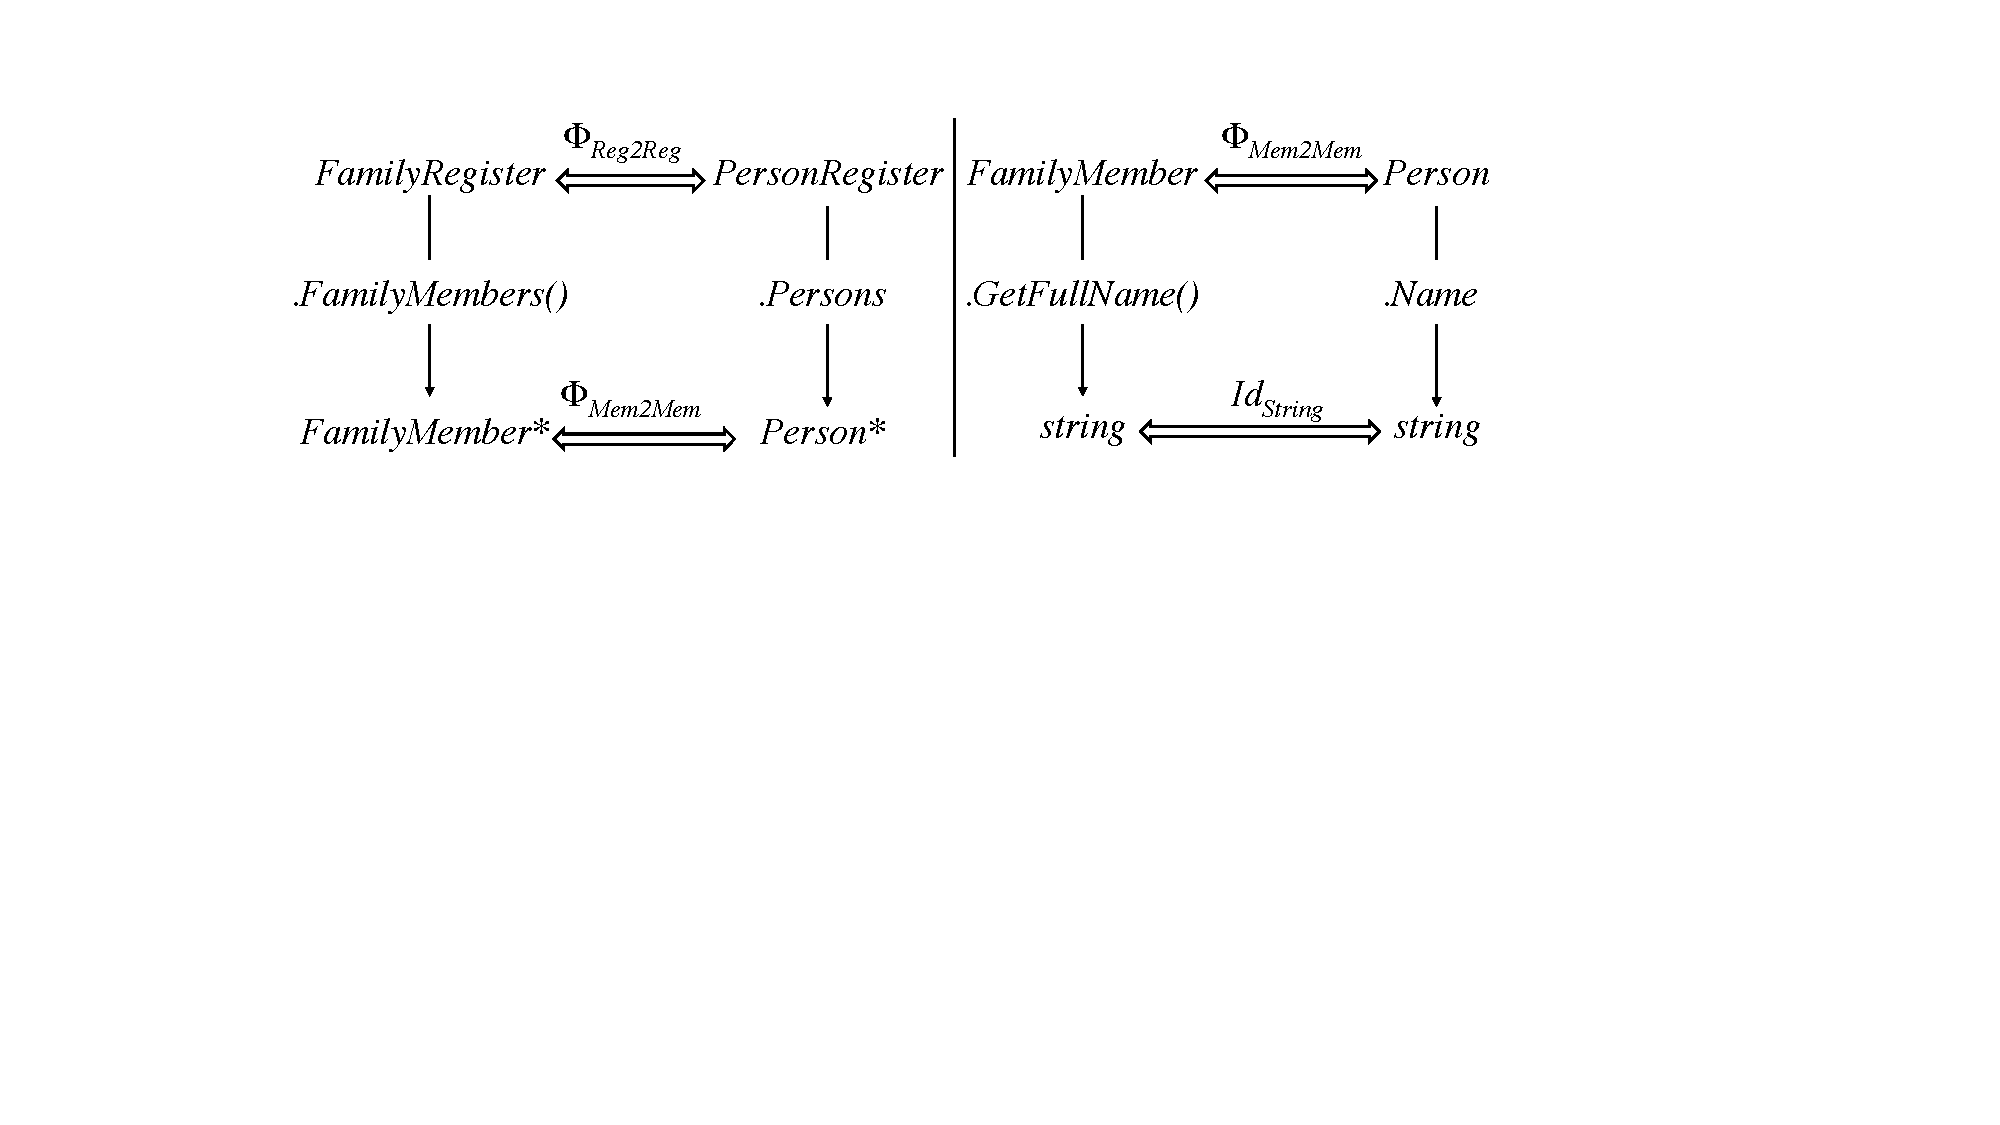
\includegraphics[width=\columnwidth]{diagrams/solutions/NMFSynchronizationBlockBenchmark}
  \caption{Synchronization blocks for benchmark solution}
  \label{fig:NMFSynchronizationBlockBenchmark}
\end{figure}

\lstdefinelanguage{cs}{
  morekeywords = {using,namespace,class,override,void,null,public,protected,private,static,out,bool,string,return,var,new,true,false,if,else,as},
  morecomment=[l]{--},
  morecomment=[s]{/*}{*/}
}

\begin{lstlisting}[label={lst:nmf}, float=b!, language=cs, caption={Solution in NMF Synchronizations}]
...
public class Reg2Reg:SynchronizationRule<
 FamilyRegister, PersonRegister>{
 public override void DeclareSynchronization(){
  SynchronizeMany(SyncRule<Mem2Mem>(),
   fam=>new FamilyMemberCollection(fam),
   persons=>persons.Persons);
 }
}
public class Mem2Mem:SynchronizationRule<
 IFamilyMember, IPerson>{
 public override void DeclareSynchronization(){
  Synchronize(m=>m.GetFullName(), p=>p.Name);
 }
}
...

private class FamilyMemberCollection 
 :CustomCollection<IFamilyMember>{
 ...
 public override void Add(IFamilyMember item){
  ...
 }
 ...
}

[LensPut(typeof(Helpers),"SetFullName")]
[ObservableProxy(typeof(Helpers),"GetFNameInc")]
public static string
 GetFullName(this IFamilyMember  member){
  return fullName.Evaluate(member);
}
public static INotifyValue<string>
 GetFNameInc(this IFamilyMember member){
  return fullName.Observe(member);
}
public static void SetFullName(
 this IFamilyMember member,
 string newName){
 ...
}
private static ObservingFunc<
 IFamilyMember,string> fullName =
  new ObservingFunc<IFamilyMember,string>
   (m=>m.Name == null ? null:
    ((IFamily)m.Parent).Name + ", " + m.Name);
...
\end{lstlisting} 

The following description of the NMF Synchronizations solution to the Families-to-Persons benchmark is based on the corresponding TTC 2017 paper~\cite{Hinkel2017}.
Two synchronization blocks are required for the transformation and are depicted in figure~\ref{fig:NMFSynchronizationBlockBenchmark}:  (i) a block with the top-level relation \emph{Reg2Reg} as base, and \emph{Mem2Mem} as target, and (ii) a block with \emph{Mem2Mem} as base and the identity relation on strings as target.

Listing~\ref{lst:nmf} depicts fragments of the solution in C\#.
The two relations are implemented as \emph{synchronization rules} subclassing the generic class \code{SynchronizationRule} (lines~2--16).
The actual synchronization blocks are defined by overriding the method \code{Declare\-Synchron\-ization} (lines~4, 12, and 18).
This is basically just a textual representation of figure~\ref{fig:NMFSynchronizationBlockBenchmark}.

Concerning the first synchronization block \code{Reg2Reg}, the target intra-model lens \code{.Persons} is simple enough (the \emph{get} function merely collects the elements obtained via a multi-valued reference) so updates (the \emph{put} function) can be inferred automatically.  
In contrast, a \emph{custom collection} \code{FamilyMember\-Collection} is required for the source intra-model lens, implemented on lines~18--25.
This helper class encapsulates the logic for determining the elements of the collection (traversing references to families and members sequentially), inserting an already created family member to the collection (line~21) at the appropriate location in the families model, depending on the configuration parameters \code{Prefer\-Existing\-To\-New\-Family} and \code{Prefer\-Parent\-To\-Child}. 

Concerning the second synchronization block \code{Mem\-2\-Mem}, the situation is similar:  the target intra-model lens \code{.Name} can be handled automatically, while the source intra-model lens \code{.Get\-Full\-Name()} has to be implemented manually on lines~27--46.
On line~27, an  annotation is used to provide \code{SetFullName} as the \emph{put} implementation for \code{GetFullName}.
The custom method \code{Set\-Full\-Name} sets the full name of a family member, potentially moving the member to a different family.

Finally, the annotation on line~28 and the implementation of the helper method \code{fullName} on lines~42--46 indicate that the NMF Synchronization framework provides hooks into infrastructure for an \emph{incrementalization} of the intra-model lens.
The reader is referred to Hinkel et al.~\cite{SoSyM2017-Hinkel} for further details.

%%% Local Variables:
%%% mode: latex
%%% TeX-master: "../main"
%%% End:
